\def\homeworknumber{4}
\def\homeworkdate{15-11-2011}

\documentclass[11pt]{article}
\linespread{1}

\renewcommand{\thefootnote}{\fnsymbol{footnote}}

\usepackage{geometry} % see geometry.pdf on how to lay out the page. There's lots.
\usepackage[utf8]{inputenc}
\usepackage{array}
\usepackage{amsmath,amssymb,latexsym,epic,eepic,epsfig,graphics,psfrag}
\usepackage{amsfonts}
\usepackage{graphicx,float}

\usepackage[danish]{babel}

\usepackage[bottom]{footmisc}

\usepackage{fancyhdr}
\pagestyle{fancy}
\lhead{\small\textit{01246 Partial Differential Equations - Fall 2011 - Anders Hørsted (s082382)}}
\rhead{\thepage}
\chead{}
\lfoot{}\cfoot{}\rfoot{}

\usepackage{pstricks}
\usepackage{pst-node}
\usepackage{wrapfig}
\usepackage{caption}
\usepackage{multirow}
%\usepackage{fouriernc}
%\usepackage[charter]{mathdesign}
\usepackage{lmodern}
\usepackage[normalem]{ulem}
\geometry{a4paper} % or letter or a5paper or ... etc
% \geometry{landscape} % rotated page geometry

\usepackage{subfigure}
\usepackage{placeins}
\usepackage{url}
\usepackage{natbib}
\renewcommand\bibsection*{}
\bibliographystyle{plain}

\makeatletter
\renewcommand*\env@matrix[1][*\c@MaxMatrixCols c]{%
  \hskip -\arraycolsep
  \let\@ifnextchar\new@ifnextchar
  \array{#1}}
\makeatother

\newcommand\myimp{\quad\Leftrightarrow\quad}
\newcommand\half{\frac{1}{2}}
%\newcommand\myvec[1]{\mathbf{#1}}
\newcommand\myvec[1]{\boldsymbol{#1}}
\newcommand\vecx{\myvec{x}}
\newcommand\mymod[1]{\ (\text{mod }#1)}
\newcommand\myreal{\mathbb{R}}
\newcommand\mynatural{\mathbb{N}}
\newcommand\myinteger{\mathbb{Z}}
\newcommand\mycomplex{\mathbb{C}}
\newcommand\myint{\text{int}}
\newcommand\norm[1]{||\,#1\,||}
\newcommand\bignorm[1]{\big|\big|\,#1\,\big|\big|}
\newcommand\seq[1]{\big\{#1\big\}}
\newcommand\smallseq[1]{\{#1\}}
\newcommand\smallseqtoinf[1]{\smallseq{#1}_{k=1}^\infty}
\newcommand\lonew{\ell^1_w}
\newcommand\lone{\ell^1}
\newcommand\ltwo{\ell^2(\mynatural)}
\newcommand\ip[2]{\langle#1,#2\rangle}
\newcommand\hilbert[1]{\mathcal{#1}}
\newcommand\uinf{u_{\infty}}
\newcommand\erf{\text{erf\,}}
\newcommand\infint{\int_{\infty}^{\infty}}
\newcommand\celsius{$^\circ$C}
\newcommand\comsol{Comsol}
\newcommand\fourier{\mathcal{F}}

\usepackage{tabulary}
\newcolumntype{y}{>{\centering\arraybackslash}R}

\setlength{\unitlength}{2mm}
\usepackage{tikz}

\title{Homework \homeworknumber}
\author{01246 Partial differential equations -- \homeworkdate -- Anders Hørsted (s082382)}
%\author{}
\date{} % delete this line to display the current date


\begin{document}
    \maketitle

    \section*{Exercise 1}

    An eigenvalue problem in $D=(0,2)^2$ is given by
    \begin{align*}
        -\Delta u &= \lambda u \text{ in } D, \\
        u &= 0 \text{ on }\partial D
    \end{align*}
    Separating variables we set $u(x, y) = X(x)Y(y)$ which gives
    \begin{align*}
        \frac{X''}{X} + \frac{Y''}{Y} = -\lambda
    \end{align*}
    Since $X$ doesn't depend on $y$ and $Y$ doesn't depend on $x$ we get from the above that 
    \begin{align*}
        X'' + k^2X = 0 \quad\text{and}\quad Y'' + l^2Y = 0
    \end{align*}
    where $\lambda = k^2+l^2$. From the boundary condition $u=0$ on $\partial D$ we get that $X(0)=X(2)=Y(0)=Y(2)=0$. For $X$ this gives
    \begin{align*}
        X = A\cos(kx) + B\sin(kx)
    \end{align*}
    Using the BC's gives
    \begin{align*}
        X(0) = A = 0 \quad\text{and}\quad X(2) = B\sin(2k) = 0 
    \end{align*}
    from which we get 
    \begin{align*}
        2k_m = m\pi \myimp k_m = \frac{m\pi}{2}
        \intertext{and}
        X_m(x)=B_m\sin(k_mx)
    \end{align*} 
    for $m=1,2,\dots$ 
    Using exactly the same procedure we also get that $Y_n(y)=D_n\sin(l_ny)$ with $l_n=\frac{n\pi}{2}$ for $n=1,2,\dots$. The eigenvalues become
    \begin{equation*}
        \lambda_{mn} = \left(\frac{m\pi}{2}\right)^2 + \left(\frac{n\pi}{2}\right)^2
    \end{equation*}
    The first eigenvalue is then given by $\lambda_1 = \lambda_{11} = \frac{\pi^2}{4} + \frac{\pi^2}{4} = \frac{\pi^2}{2}$ and the corresponding eigenfunction is then
    \begin{align*}
        w_1(x,y) &= c\sin\left(k_1x\right)\sin\left(l_1y\right)\\
            &= c\sin\left(\frac{\pi}{2}x\right)\sin\left(\frac{\pi}{2}y\right)
    \end{align*}
    with $c=B_mD_n$. \\\\
    
    \noindent The constant $c$ is now chosen such that $\iint_D |w_1|^2\,dxdy=1$. By insertion
    \begin{align*}
        \iint_D \left|c\sin\left(\frac{\pi}{2}x\right)\sin\left(\frac{\pi}{2}y\right)\right|^2\, dxdy = 1
    \end{align*}
    and since $\sin\left(\frac{\pi}{2}x\right)\sin\left(\frac{\pi}{2}y\right)\geq0$ for $(x,y)\in D$ we get
    \begin{align*}
        c^2 &= \frac{1}{\iint_D \sin^2\left(\frac{\pi}{2}x\right)\sin^2\left(\frac{\pi}{2}y\right)\,dxdy} \\
            &= 1
    \end{align*}
    so in principle $c=\pm 1$, but since $c$ is a normalization constant we choose $c=1$.


    \section*{Question 2}

    We continue to look at the PDE problem from question 1, but now use FEM to approximate $\lambda_1$ and $w_1$ numerically. The square $D=[0,2]^2$ is therefore divided into four triangles by the two diagonals (see figure~\ref{fig:mesh}), giving a mesh with one interior point $(1,1)$ and the corresponding test function $v_1$. Using $v_1$ we approximate $w_1$ by $u_1 = U_1v_1$ where $U_1\neq 0$.

    \begin{figure}
        \centering
        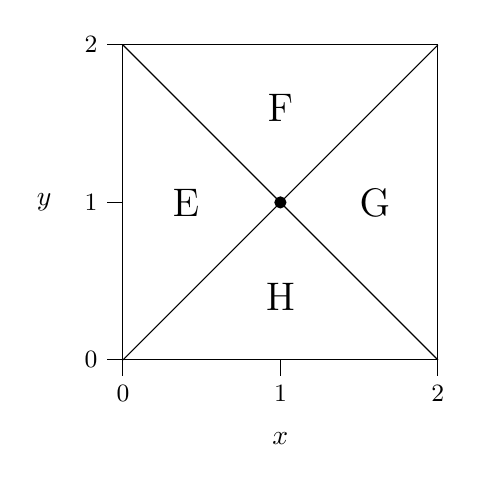
\begin{tikzpicture}
\draw (1,1) rectangle (5,5);
\draw (1,1) --(5,5);
\draw (1,5) --(5,1);
\draw (1,.8) -- (1,1);
\node [below] at (1,.8) {\small 0};
\draw (3,.8) -- (3,1);
\node [below] at (3,.8) {\small 1};
\draw (5,.8) -- (5,1);
\node [below] at (5,.8) {\small 2};
\draw (.8,1) -- (1,1);
\node [left] at (.8,1) {\small 0};
\draw (.8,3) -- (1,3);
\node [left] at (.8,3) {\small 1};
\draw (.8,5) -- (1,5);
\node [left] at (.8,5) {\small 2};
\node at (1.8,3) {\Large E};
\node at (3,4.2) {\Large F};
\node at (4.2,3) {\Large G};
\node at (3,1.8) {\Large H};
\node at (3,0) {$x$};
\node at (0,3) {$y$};
\draw[fill] (3,3) circle(0.07);
%\draw (3.05,2.6) node {$v_1$};
\end{tikzpicture}

        \hspace{8mm}
        \caption{Mesh for the FEM calculations in question 2}
        \label{fig:mesh}
    \end{figure}

    \subsection*{a)}

    The test function $v_1$ is determined. $v_1$ should equal 1 at the vertex $(1,1)$ and 0 at the boundary. Also $v_1=a+bx+cy$ is linear with different $a,b,c$ in each triangle. Looking at triangle $E=\{(x,y)|x\in[0,1], x\leq y \leq 2-x\}$ we call $v_1$ constrained to $E$ for $v_{E}$. Then
    \begin{gather*}
        v_E(0,y) = a_E + c_Ey = 0 \quad \Rightarrow \quad a_E=c_E=0
        \intertext{and}
        v_E(1,1) = a_E + b_E + c_E = b_E = 1 
    \end{gather*}
    which gives $v_E(x,y)=x$. For triangle $F$ we get
    \begin{gather*}
        v_F(x,2) = a_F + b_Fx + 2c_F = 0 \quad \Rightarrow \quad b_F = 0 \,\land\, a_F+2c_F = 0
        \intertext{and}
        v_F(1,1) = a_F + b_F + c_F = a_F + c_F = 1
    \end{gather*}
    Combining $a_F+c_F=1$ and $a_F+2c_F=0$ gives $a_F=2$ and $c_F=-1$ which gives $v_F(x,y)=2-y$.

    Using the same procedure for $G$ and $H$ gives
    \begin{equation*}
        v_1(x,y) = \begin{cases}
            x & (x,y)\in E \\
            2-y & (x,y)\in F \\
            2-x & (x,y)\in G \\
            y & (x,y)\in H
        \end{cases}
    \end{equation*}

    \subsection*{b)}

    Using FEM the equation
    \begin{equation}\label{eq:FEM}
        U_1M_{11} = \lambda U_1K_{11}
    \end{equation}
    is derived and $M_{11}$ and $K_{11}$ are calculated. First the eigenvalue problem in question 1 is multiplied by the test function $v_1$ giving
    \begin{align*}
        -\Delta uv_1 &= \lambda uv_1 \\
        -\iint_D \Delta uv_1\, dxdy &= \lambda\iint_D uv_1\, dxdy
    \end{align*}
    Using Green's first identity and that $v_1=0$ on $\partial D$ gives
    \begin{align*}
        \iint_D \nabla u \nabla v_1\, dxdy &= \lambda\iint_D uv_1\, dxdy
    \end{align*}
    and then substituting $u = U_1v_1$
    \begin{align*}
        U_1\iint_D |\nabla v_1|^2 \, dxdy &= \lambda U_1\iint_D v_1^2\, dxdy
    \end{align*}
    Setting $M_{11}=\iint_D |\nabla v_1|^2 \, dxdy$ and $K_{11}=\iint_D v_1^2\, dxdy$ gives equation (\ref{eq:FEM}).

    Since
    \begin{equation*}
        \nabla v_1 = \begin{cases}
            [1 \quad 0] & (x,y)\in E \\
            [0 \quad -1] & (x,y)\in F \\
            [-1 \quad 0] & (x,y)\in G \\
            [0 \quad 1] & (x,y)\in H
        \end{cases}
    \end{equation*}
    we have that $|\nabla v_1|=1$ for $(x,y)\in D$ and therefore
    \begin{align*}
        M_{11} &= \iint_D 1 \, dxdy \\
        &= 4
    \end{align*}
    Using the symmetry of $v_1$ we get
    \begin{align*}
        K_{11} &= \iint_D v_1^2\, dxdy \\
        &= 8\int_0^1\int_0^x y^2\, dydx \\
        &= \frac{2}{3}
    \end{align*}

    \subsection*{c)}

    Using the calculated values for $M_{11}$ and $K_{11}$ we solve for $\lambda$ which gives
    \begin{align*}
        4 U_1 &= \lambda \frac{2}{3}U_1 \myimp\\
        \lambda &= 6
    \end{align*}
    Compared with the first eigenvalue found analytically $\lambda_1=\frac{\pi^2}{2}\approx 4.93$ the approximated value is seen to be a bit above. That the approximated eigenvalue is a bit off is probably due to the coarse mesh.

    \subsection*{d)}

    The approximation $u_1$ is now found by the constraint $\iint_D |u_1|^2\, dxdy = 1$. Since
    \begin{align*}
        \iint_D |u_1|^2\, dxdy &= |U_1|^2\iint_D v_1^2\, dxdy \\
        &= \frac{2}{3}U_1^2 
    \end{align*}
    we get
    \begin{align*}
        \frac{2}{3}U_1^2 &= 1 \myimp \\
        U_1 &= \pm \sqrt{\frac{3}{2}}
    \end{align*}
    so we get 
    \begin{equation*}
        u_1 = \sqrt{\frac{3}{2}}\,v_1
    \end{equation*}

    \begin{figure}[ht]
        \centering
        \includegraphics[width=120mm]{diff-fem.png}
        \caption{Difference between the analytical found eigenfunction $w_1$ and the approximated function $u_1$}
        \label{fig:diff-fem}
    \end{figure}


    \section*{Question 3}

    A beef roast is in the shape of a sphere with radius 8cm. It has an initial temperature of 5\celsius\ and is put in the oven, which has a temperature of 200\celsius. The heat conduction of beef is given as $k=1.1\cdot 10^{-3}\text{cm}^2/\text{s}$. 

    \subsection*{a)}

    The shape of the beef is modelled as $D=B(0,8)$ a ball of radius 8cm and $u(x,t)$ is the temperature at time $t>0$ and point $x\in D$. Letting the specific heat and the density of the beef be constant, the heat equation becomes the diffusion equation, so we should expect $u$ to satisfy the diffusion equation. The initial temperature is 5\celsius\ so $u=5$ at time $t=0$. Since the oven is 200\celsius\ this should also be true for the surface of $D$, so $u=200$ at $\partial D$. The conditions combined gives the boundary value problem
    \begin{align}
        u_t - k\Delta u &= 0 \text{ in } D, \nonumber\\
        u &= 5 \text{ at } t=0, \label{eq:pde-beef}\\
        u &= 200 \text{ on } \partial D \nonumber
    \end{align}

    \subsection*{b)}

    The PDE problem (\ref{eq:pde-beef}) is solved for $u$. To obtain homogeneous boundary conditions a new function is defined as $v=u-200$ and it should fulfill
    \begin{align*}
        v_t - k\Delta v &= 0 \text{ in } D,\\
        v &= -195 \text{ at } t=0, \\
        v &= 0 \text{ on } \partial D 
    \end{align*}
    This is the diffusion equation in the ball of radius 8 with homogeneous BC and the general solution is given in equation 10.3.22 in the course textbook as
    \begin{equation*}
        v(r,\theta,\phi,t) = \sum_{l=0}^\infty\sum_{j=1}^\infty\sum_{m=-l}^{l} A_{lmj} e^{-k\lambda_{lj}t}\frac{J_{l+1/2}(\sqrt{\lambda_{lj}}r)}{\sqrt{r}}P_l^{|m|}(\cos\theta)e^{im\phi}
    \end{equation*}
    Due to the symmetry of $D$ and the initial condition we assume that $v$ is independent of $\theta$ and $\phi$ which corresponds to setting $l=m=0$ and only sum over $j$. The solution is then
    \begin{equation*}
        v(r,t) = \sum_{j=1}^\infty A_{j} e^{-k\lambda_{j}t}\frac{J_{1/2}(\sqrt{\lambda_{j}}r)}{\sqrt{r}}
    \end{equation*}
    where the eigenvalues $\lambda_j$ are the solutions to the equation
    \begin{align*}
        J_{1/2}(8\sqrt{\lambda_j}) = \sqrt{\frac{1}{4\pi\sqrt{\lambda_j}}}\sin(8\sqrt{\lambda_j}) = 0
    \end{align*}
    and therefore
    \begin{align*}
        8\sqrt{\lambda_j} = j\pi \myimp \lambda_j = \left(\frac{j\pi}{8}\right)^2
    \end{align*}
    To determine $A_j$ we use the initial condition and the fact that the eigenfunctions $w_j(r) = \frac{J_{1/2}(\sqrt{\lambda_j}r)}{\sqrt{r}}$ are orthogonal and then find
    \begin{align*}
        A_j &= \frac{\iiint_D -195\cdot\frac{J_{1/2}(\sqrt{\lambda_j}r)}{\sqrt{r}}\,d\vecx}{\iiint_D \left|\frac{J_{1/2}(\sqrt{\lambda_j}r)}{\sqrt{r}}\right|^2\,d\vecx} \\
        &= \frac{-195\int_0^8\int_0^\pi\int_0^{2\pi} \sqrt{\frac{1}{r}}\sqrt{\frac{16}{\pi^2jr}}\sin(\frac{\pi j}{8}r)\,r^2\sin(\theta)\,d\phi d\theta dr}{\int_0^8\int_0^\pi\int_0^{2\pi} \left(\sqrt{\frac{1}{r}}\sqrt{\frac{16}{\pi^2jr}}\sin(\frac{\pi j}{8}r)\right)^2r^2\sin(\theta)\,d\phi d\theta dr} \\
        &= \frac{-195\int_0^8\sin(\frac{\pi j}{8}r)\,r\,dr}{\frac{4}{\pi\sqrt{j}}\int_0^8\sin^2(\frac{\pi j}{8}r)\,dr} \\
        &= (-1)^j\frac{780}{\sqrt{j}}
    \end{align*}
    which gives
    \begin{align*}
        v(r,t) &= \sum_{j=1}^\infty\,(-1)^j\frac{780}{\sqrt{j}}\,e^{-kj^2\pi^2 t/64}\,\frac{J_{1/2}\left(\frac{j\pi r}{8}\right)}{\sqrt{r}}\\
        &= 3120\sum_{j=1}^\infty\,(-1)^j\,e^{-kj^2\pi^2 t/64}\,\frac{\sin\left(\frac{j\pi r}{8}\right)}{j\pi r}
    \end{align*}
    and then
    \begin{align*}
        u(r,t) = 200 + v(r,t)
    \end{align*}

    \subsection*{c)}

    The solution $u$ is now approximated by
    \begin{equation}\label{eq:truncated}
        u_N(r,t) = 200 + 3120\sum_{j=1}^N\,(-1)^j\,e^{-kj^2\pi^2 t/64}\,\frac{\sin\left(\frac{j\pi r}{8}\right)}{j\pi r}
    \end{equation}
    where we choose $N=100$ and then plot $u_N(0,t)$ to find $T$ such that $u_N(0,T)=58$. The plot is shown in figure~\ref{fig:timeplots-u} and it is seen that $T\approx 5600\,\text{s}$.

    \begin{figure}
        \centering
        \mbox{\subfigure{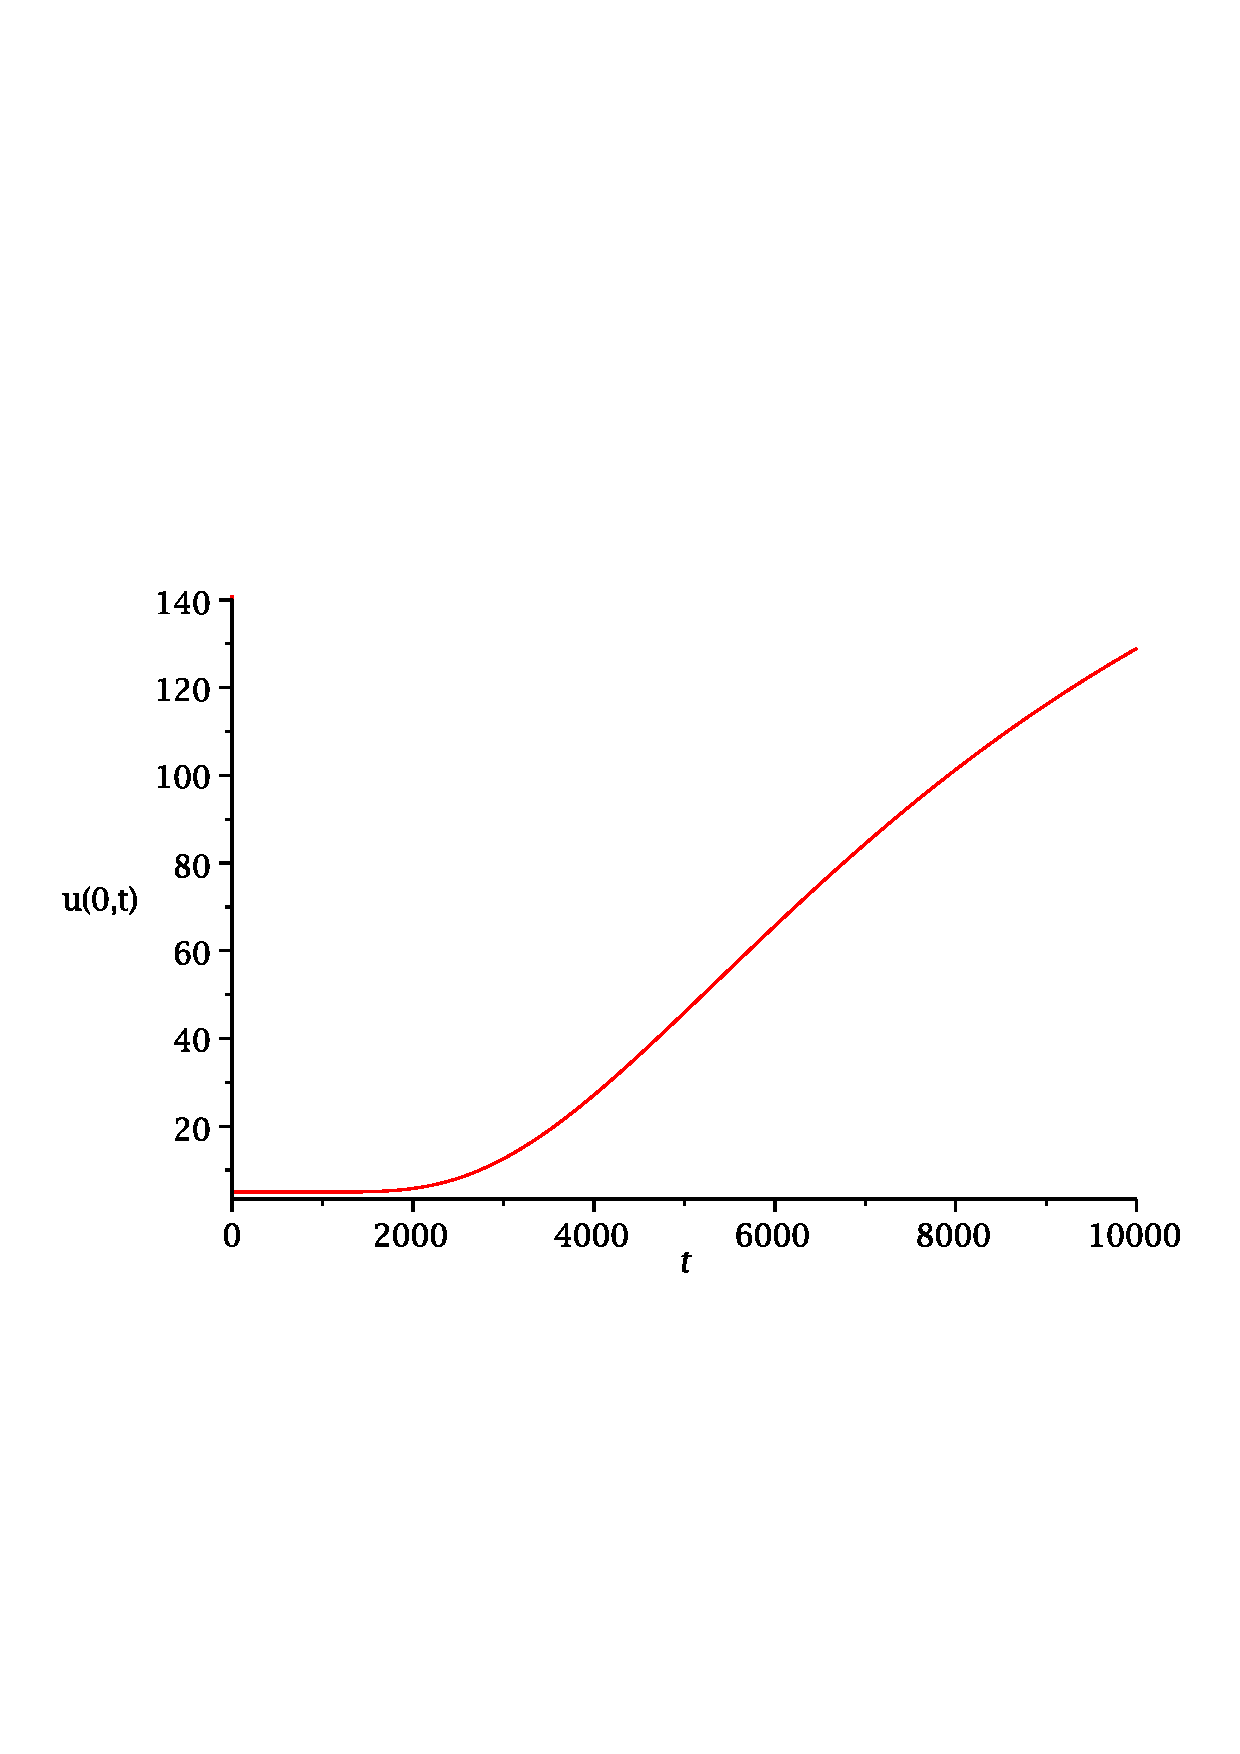
\includegraphics[width=70mm]{timeplot-u.pdf}} \quad 
            \subfigure{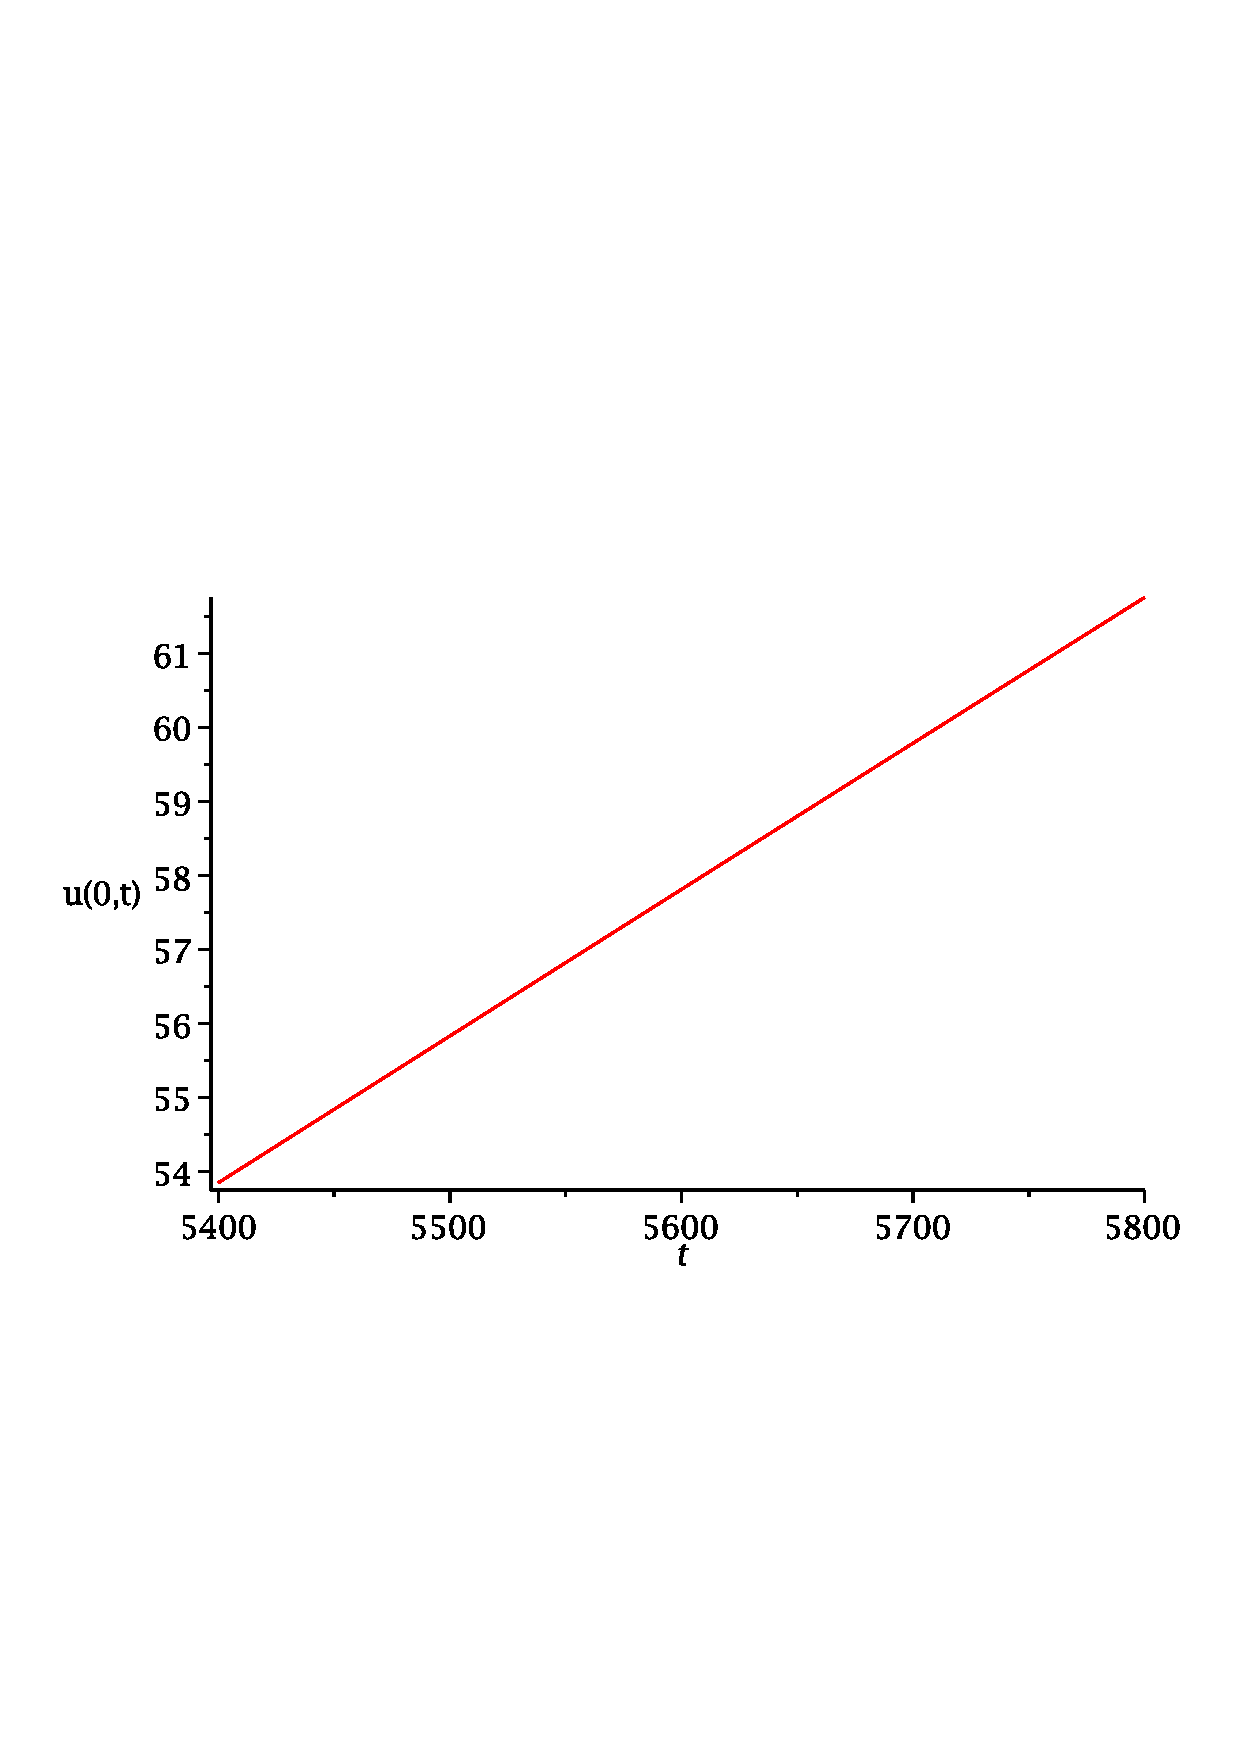
\includegraphics[width=70mm]{timeplot-u-2.pdf}}}
        \caption{Plots of the temperature at the center of the roast beef for different times, calculated using the truncated series (\ref{eq:truncated}) with $N=100$.}
        \label{fig:timeplots-u}
    \end{figure}

    \subsection*{d)}

    The boundary value problem for the roast beef is now solved numerically using \comsol. A new model is created in \comsol\ by using the model wizard. First ``3D'' is selected as space. Then the ``Heat Equation'' is chosen from the ``Classical PDEs''. The ``Time Dependent'' study type is chosen and the wizard is finished. Then a sphere with radius $0.08$m is build. Under ``Heat Equation'' the constant $c$ is set to $1.1\cdot10^{-7}\,\text{m}^2/\text{s}$ and the Dirichlet Boundary Condition is added. The model is computed and two 3D-plots of the sphere at time $t=T=5600$ are plotted and shown in figure~\ref{fig:comsol}. One plot shows three slices and the other shows five slices. From the plots it is seen that the temperature is low in the center and then graduately becomes warmer as the boundary is approached. Also the coldest point seems to be the center and from the colorbar it is seen to be approximately 58\celsius.

    \begin{figure}
    \centering
    \mbox{\subfigure{\includegraphics[width=70mm]{t-5600-slices-3.png}} \quad 
        \subfigure{\includegraphics[width=70mm]{t-5600-slices-5.png}}}
    \caption{Comsol plots of the roast beef at time $t=T=5600$}
    \label{fig:comsol}
    \end{figure}

    \subsection*{e)}

    In cookbooks the time to prepare a roast beef is often estimated to be around 1.5 hours. Comparing this advice to the result that the center is 58\celsius at time $T=5600\,\text{s}$ is seen to match pretty well since
    \begin{equation*}
        5600\,\text{s} \cdot \frac{1}{3600}\,\frac{\text{h}}{\text{s}} \approx 1.56\,\text{h}
    \end{equation*}

\end{document}
